\documentclass[12pt]{article}
\renewcommand{\baselinestretch}{1.1}

%%% Add packages here
\usepackage{graphicx} 
\usepackage{parskip}
\usepackage[table]{xcolor}
\usepackage{amsmath}
\usepackage{float}
\usepackage{geometry}
\geometry{legalpaper, portrait, margin=3cm}
\usepackage{makecell}
\usepackage{multirow}
\usepackage{array}
\usepackage{amsfonts}
\usepackage{amsthm}
\usepackage{amssymb}
\usepackage{latexsym}
\usepackage{color}
\usepackage{verbatim}
\usepackage{fancyhdr}
\usepackage{fancybox}
\usepackage{listings}
\usepackage{threeparttable} % for table notes
\usepackage{hologo} % for TeX engine logos
\usepackage{booktabs} % for nice tables
\usepackage{longtable} % for longer tables
\usepackage[table,xcdraw]{xcolor}  % for color in tables
\usepackage{appendix} % for appendix
\usepackage{biblatex}
\addbibresource{references.bib}

\usepackage{amsmath} % for pseudo code
\usepackage{algorithm}
\usepackage{algpseudocode}

%%% Margins
\addtolength{\oddsidemargin}{-.50in}
\addtolength{\evensidemargin}{-.50in}
\addtolength{\textwidth}{1.0in}
\addtolength{\topmargin}{-.40in}
\addtolength{\textheight}{0.80in}

%%% Header
\pagestyle{fancy}
\chead{} % Clear undefined \groupname
\rhead{}
\lhead{}
\cfoot{\thepage}
\renewcommand{\headrulewidth}{0.4pt}

%%%%%%%%%%%%%%%%%%%%%%%%%%%%%%%%%%%%%

\begin{document}
\clearpage\thispagestyle{empty}

\begin{titlepage}

\begin{center}
\vspace*{1in}
	% title
	\centering\textbf{\huge{Bayesian data analysis project\\[1cm]
 }} \\[2cm]
	% details
	\Large{
	Master of Statistics and Data Science \\
	Hasselt University\\	
        2024-2025 \\
	}


\vspace*{3cm}
\textbf{\large{Group :}}\\
Luong Vuong (2365900) \\
Edward Owinoh (2365191) \\
Joseph Kaunda (2364031) \\



\vspace*{2cm}


\vspace*{1.5cm}
\textbf{\large{Lecturers:}}\\
Prof. Dr. Christel Faes \\
Dr. Oswaldo Gressani \\


\vspace*{2\baselineskip}
\today

\begin{figure}[b]
   \centering
   
\includegraphics[width=8cm]{pictures/UHasselt_logog.png}
   \label{fig:Uhasselt}
\end{figure}

\end{center}

\end{titlepage}

\section{Part 1}

\section{Part 2 - The Gibbs algorithm}
Let \(\boldsymbol{\theta} = (\theta_1, \theta_2)^\top \in \mathbb{R}^2\) and consider the following (unscaled) posterior density:

\[
p(\boldsymbol{\theta} \mid \mathcal{D}) \propto \exp\left(-8\theta_1^2\theta_2^2 - 0.5\theta_1^2 - 0.5\theta_2^2 + \cos(2\pi + 0.3)\theta_1\theta_2 + 0.3\theta_1 + 0.2\theta_2 \right).
\]

\subsection{Derive the conditional posteriors \(p(\theta_1 \mid \theta_2, \mathcal{D})\) and \(p(\theta_2 \mid \theta_1, \mathcal{D})\). To what well-known parametric family do these conditional posterior distributions belong? Explain mathematically how you computed the conditional posterior mean \(E(\theta_1 \mid \theta_2, \mathcal{D})\) and the conditional posterior variance \(V(\theta_1 \mid \theta_2, \mathcal{D})\).} 
\subsubsection{Solution \(p(\theta_1 \mid \theta_2, \mathcal{D})\) }{\label{theta1}}
We first focus on deriving the conditional posterior of  \(p(\theta_1 \mid \theta_2, D)\) using the steps below:

\begin{enumerate}
\item Re-arranging terms from the joint posterior density with respect to $\theta_1$ terms we get:

\begin{equation}\label{theta1eq1}
p(\theta \mid \mathcal{D}) \propto \exp \left( -8\theta_1^2\theta_2^2 - 0.5\theta_1^2 + \theta_1(\cos(2\pi + 0.3)\theta_2 + 0.3) \right) \times \exp \left( -0.5\theta_2^2 + 0.2\theta_2 \right)  
\end{equation} 
\item Since  $\exp \left( -0.5\theta_2^2 + 0.2\theta_2 \right)$  is not a function dependent on $\theta_1$ in eqn  \ref{theta1eq1}, $p(\theta_1 \mid \theta_2 ,\mathcal{D}) $ can then be written as:
 \begin{equation}\label{theta1eq2}
p(\theta_1 \mid \theta_2 ,\mathcal{D}) \propto \exp \left( -8\theta_1^2\theta_2^2 - 0.5\theta_1^2 + \theta_1(\cos(2\pi + 0.3)\theta_2 + 0.3) \right)
\end{equation} 

This is a quadratic function of $\theta_1$ and can be rewritten as   \begin{equation}\label{theta1eq3}
p(\theta_1 \mid \theta_2 ,\mathcal{D}) \propto \exp\left[- \frac{1}{2}\left( 16\theta_1^2\theta_2^2 + \theta_1^2 - 2*(\cos(2\pi + 0.3)\theta_2 \theta_1) - 2*(0.3\theta_1 \right)\right]
\end{equation} 

\item We arrange the exponent in equation \ref{theta1eq3} according to power terms of $\theta_1$ and define $X$ and $Y$ as shown in equation \ref{condtheta1}:
\begin{equation}\label{condtheta1}
-\frac{1}{2} \left( \underbrace{(16\theta_2^2 + 1)}_{X}\theta_1^2 - 2\underbrace{\left(\cos(2\pi + 0.3)\theta_2 + 0.3\right)}_{Y}\theta_1 \right)
\end{equation}

\item Using the completing square method we can rewrite the terms in the brackets in equation \ref{condtheta1} as 

\begin{equation}\label{condtheta2}
     X\theta_1^2 - 2Y\theta_1 = X\left(\theta_1 - \frac{Y}{X}\right)^2 - \frac{Y^2}{X}
\end{equation} from which $\left(\theta_1 - \frac{Y}{X}\right)^2$ is the kernel of a Gaussian distribution for (that could generally be written as)  $\theta_1 \sim \mathcal{N} \left(\frac{Y}{X}, \frac{1}{X} \right)$
\item Substituting \( X = 16\theta_2^2 + 1 \) and \( Y = \cos(2\pi + 0.3)\theta_2 + 0.3 \) in eqn \ref{condtheta2} the full conditional posterior density  can be written as:

\begin{equation} \label{condtheta3}
p(\theta_1 \mid \theta_2, \mathcal{D}) \propto \exp\left[-\frac{1}{2}(16\theta_2^2 + 1)\left(\theta_1 - \frac{\cos(2\pi + 0.3)\theta_2 + 0.3}{16\theta_2^2 + 1}\right)^2\right]
\end{equation}

We can then conclude from equation \ref{condtheta3} that
\begin{equation}\label{condtheta4}
\theta_1 \mid \theta_2, D \sim \mathcal{N} \left( \frac{\cos(2\pi+0.3)\theta_2 + 0.3}{1 + 16\theta_2^2}, \frac{1}{1 + 16\theta_2^2} \right)
\end{equation}
\end{enumerate}



\subsubsection{Solution \(p(\theta_2 \mid \theta_1, \mathcal{D})\) }
To derive the conditional posterior \(p(\theta_2 \mid \theta_1, \mathcal{D})\), we repeat the steps in section \ref{theta1} but with a focus on $\theta_2$:

\begin{enumerate}
    \item From the joint posterior density we re-arrange the equation w.r.t $\theta_2$ terms as:
\begin{equation}\label{theta2eq1}
p(\theta \mid \mathcal{D}) \propto \exp \left( -8\theta_1^2\theta_2^2 - 0.5\theta_2^2 + \theta_2(\cos(2\pi + 0.3)\theta_1 + 0.2) \right) \times \exp \left( -0.5\theta_1^2 + 0.3\theta_1 \right) 
\end{equation} 
\item Since  $\exp  \left( -0.5\theta_1^2 + 0.3\theta_1 \right)$  is not a function dependent on $\theta_2$ in equation  \ref{theta2eq1}, $p(\theta_2 \mid \theta_1 ,\mathcal{D}) $ can then be written as:
 \begin{equation}\label{theta2eq2}
p(\theta_2 \mid \theta_1 ,\mathcal{D}) \propto \exp \left( -8\theta_1^2\theta_2^2 - 0.5\theta_2^2 + \theta_2(\cos(2\pi + 0.3)\theta_1 + 0.2) \right)
\end{equation} 
a quadratic function of $\theta_2$ and could then be rewritten as:
 \begin{equation}\label{theta2eq3}
p(\theta_2 \mid \theta_1 ,\mathcal{D}) \propto \exp\left[- \frac{1}{2}\left( 16\theta_1^2\theta_2^2 + \theta_2^2 - 2*(\cos(2\pi + 0.3)\theta_2 \theta_1) - 2*(0.2\theta_2 \right)\right]
\end{equation}

\item From literature \cite{gelman1995bayesian} \cite{author2024notes}, if you have a conditional prior in the form of 
 \begin{equation}\label{theta2eq4}
p(\theta_2 \mid \theta_1, \mathcal{D}) \propto \exp\left\{ -\frac{1}{2} \left( A\theta_1^2\theta_2^2 + \theta_2^2 - 2B\theta_1\theta_2 - 2C_2\theta_2 \right) \right\}
\end{equation}
 this implies that $\theta_2 \mid \theta_1, \mathcal{D} \sim \mathcal{N} \left( \frac{B\theta_1 + C_2}{1 + A\theta_1^2}, \frac{1}{1 + A\theta_1^2} \right)$.
\item Substituting this in equation \ref{theta2eq3}, then we can conclude that $\theta_2 \mid \theta_1, \mathcal{D} \sim \mathcal{N} \left( \frac{\cos(2\pi + 0.3)\theta_1 + 0.2}{16\theta_1^2 + 1}, \frac{1}{16\theta_1^2 + 1}\right)$.   
\end{enumerate}

\textbf{Summary} \\
We have shown that both conditional distributions are Gaussian (normal), a subclass of the exponential family with $\theta_1 \mid \theta_2, D \sim \mathcal{N} \left( \frac{\cos(2\pi+0.3)\theta_2 + 0.3}{1 + 16\theta_2^2}, \frac{1}{1 + 16\theta_2^2} \right)$ and $\theta_2 \mid \theta_1, \mathcal{D} \sim \mathcal{N} \left( \frac{\cos(2\pi + 0.3)\theta_1 + 0.2}{16\theta_1^2 + 1}, \frac{1}{16\theta_1^2 + 1}\right)$

\subsubsection{Conditional posterior mean \(E(\theta_2 \mid \theta_1, \mathcal{D})\) and the conditional posterior variance \(V(\theta_1 \mid \theta_2, \mathcal{D})\).}

We can mathematically derive the conditional posterior mean and variance as described from equations \ref{theta1eq1} - \ref{condtheta4}.  From $\theta_1 \mid \theta_2, D \sim \mathcal{N} \left( \frac{\cos(2\pi+0.3)\theta_2 + 0.3}{1 + 16\theta_2^2}, \frac{1}{1 + 16\theta_2^2} \right)$ we conclude
$\mathbb{E}(\theta_1 \mid \theta_2, \mathcal{D}) = \frac{\cos(2\pi + 0.3)\theta_2 + 0.3}{16\theta_2^2 + 1}$ and variance  $  \mathrm{Var}(\theta_1 \mid \theta_2, \mathcal{D}) = \frac{1}{16\theta_2^2 + 1}$

\subsection{ Based on the full conditionals obtained in the previous step, write a pseudo-code to obtain a random sample of total size 50,000 (including a burn-in of size 20,000) from $p(\theta | \mathcal{D})$ using the Gibbs sampler.} 
\subsubsection{Solution}


The full two stage Gibbs sample pseudo-code is as shown below:
\begin{algorithm}
\begin{algorithmic}[1]
\State Fix initial values \( \theta_1 = \theta_1^{(0)} \), \( \theta_2 = \theta_2^{(0)} \).
\For{\( i = 1 \), \ldots , \( 50000 \)}
    \State Sample \( \theta_1^{(i)} \sim \mathcal{N}\left(\frac{\cos(2\pi + 0.3)\theta_2^{(i-1)} + 0.3}{16(\theta_2^{(i-1)})^2 + 1)}, \frac{1}{2(8(\theta_2^{(i-1)})^2 + 1)}\right) \).
    \State Sample \( \theta_2^{(i)} \sim \mathcal{N}\left(\frac{\cos(2\pi + 0.3)\theta_1^{(i)} + 0.2}{16(\theta_1^{(i)})^2 + 1)}, \frac{1}{16(\theta_1^{(i)})^2 + 1)}\right) \).
\EndFor
\State Discard the first \( b = 20,000 \) samples as burn-in
\State Return \( \{\theta_1^{(i)}, \theta_2^{(i)}\}_{i=B+1}^{N} \) which under mild regularity and if convergence occurs can be said to be drawn from \( p(\boldsymbol{\theta} \mid \mathcal{D}) \).
\end{algorithmic}
\caption{ Gibbs Sampler to draw from \( p(\boldsymbol{\theta} \mid \mathcal{D}) \)}
\label{algo:gs}
\end{algorithm}

\subsection{Using R and without relying on external software/packages (except the \texttt{coda} package), write the Gibbs sampler based on your pseudo-code in step 2. Please specify \texttt{set.seed(2025)} at the beginning of your code for reproducibility of your results. What is your acceptance rate?}
\subsubsection{Solution}
Gibbs sampling was performed for 50000 iterations  as stated in the pseudo-code  "Algorithm \ref{algo:gs}." The initial values for $\theta_1 \& \theta_2$ were set to 0.1. The first 20,000 samples were discarded as burn-in and the resulting chain analysed using histograms, trace plots, and summary statistics, including means, medians, 95\% HDP intervals, and 95\% equal-tail credible intervals as shown in Figure \ref{fig:gs-histogram} , Figure \ref{fig:gs-traceplot} and Table \ref{tab:summary_gs} respectively.

\begin{figure}[h!]
    \centering
    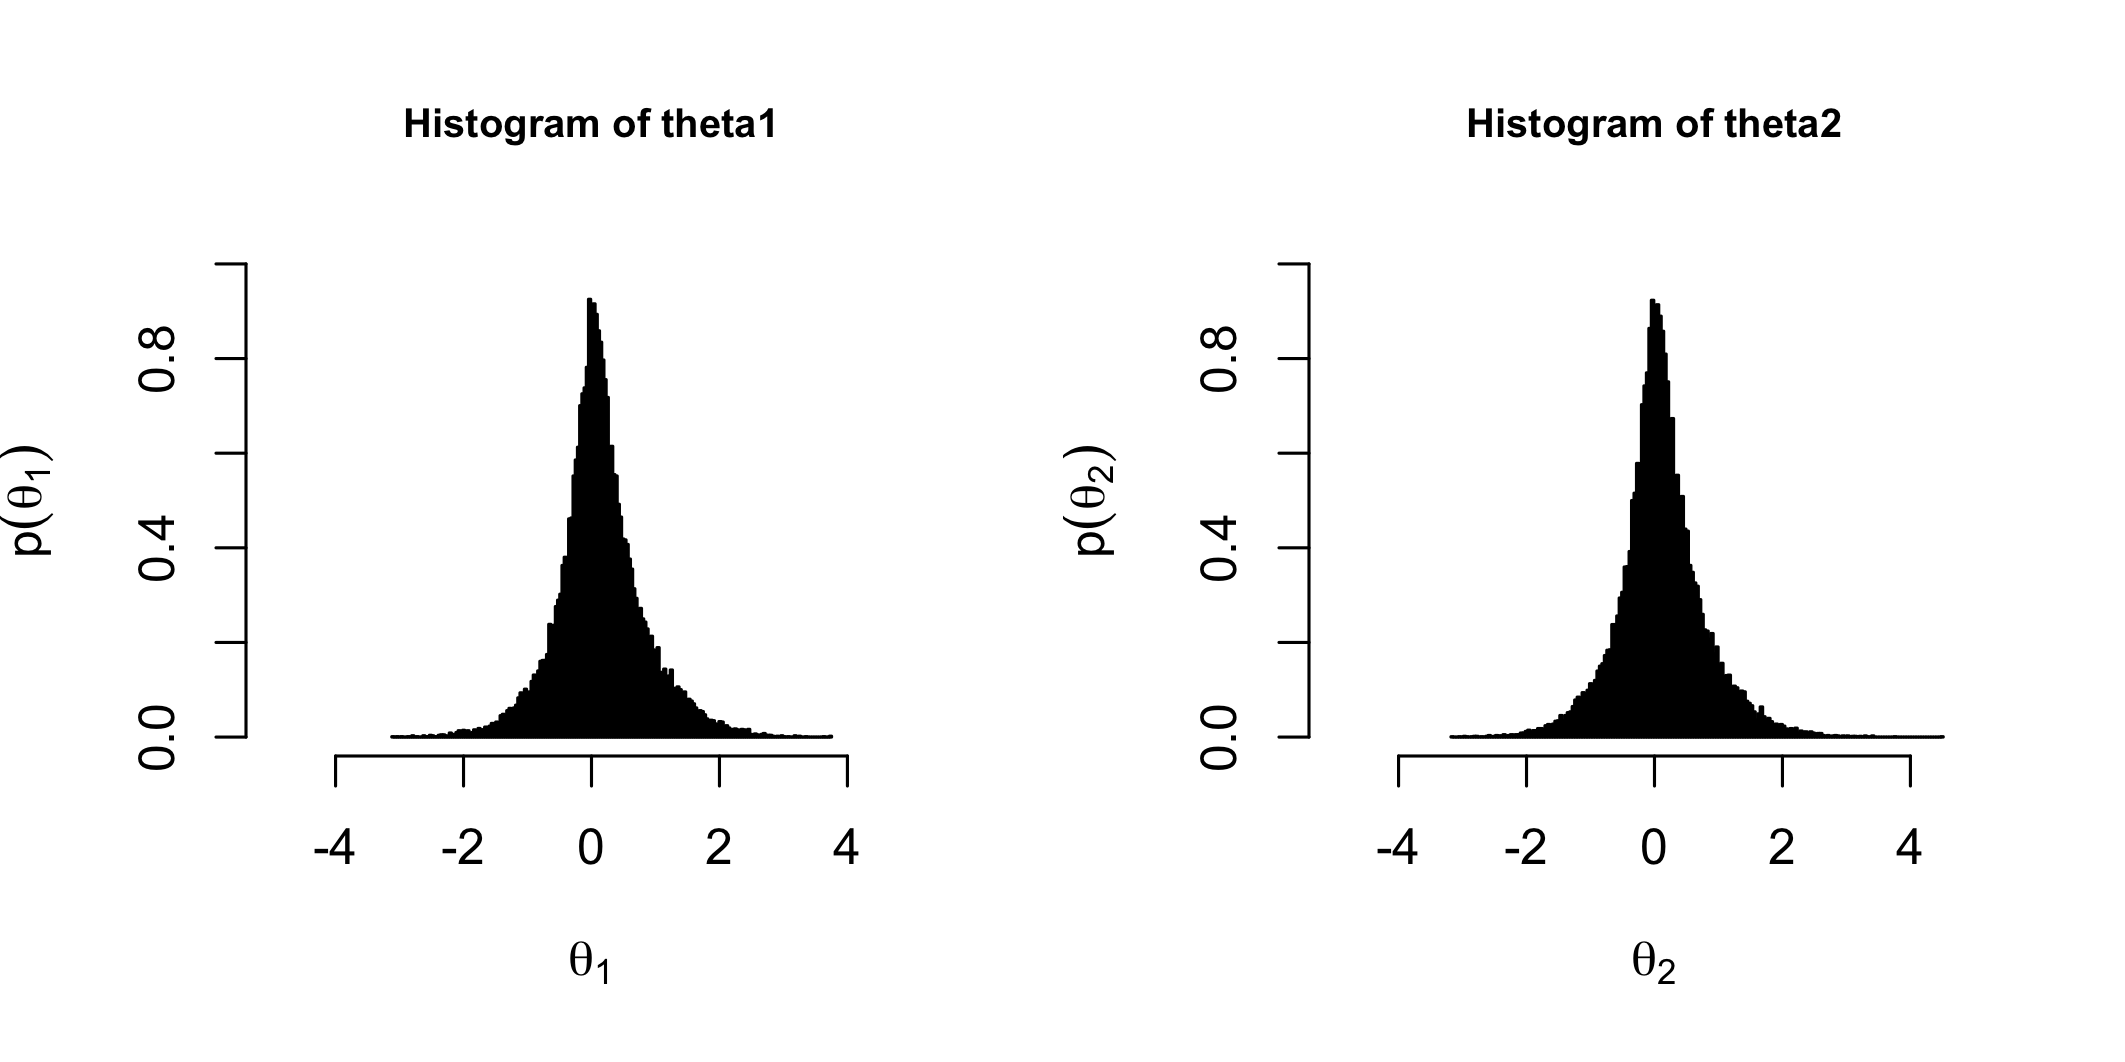
\includegraphics[width=0.6\linewidth]{pictures/fig02-gs-histogram.png}
    \caption{Sampling Histograms for $\theta_1$ and $\theta_2$ }
    \label{fig:gs-histogram}
\end{figure}

\begin{figure}[h!]
    \centering
    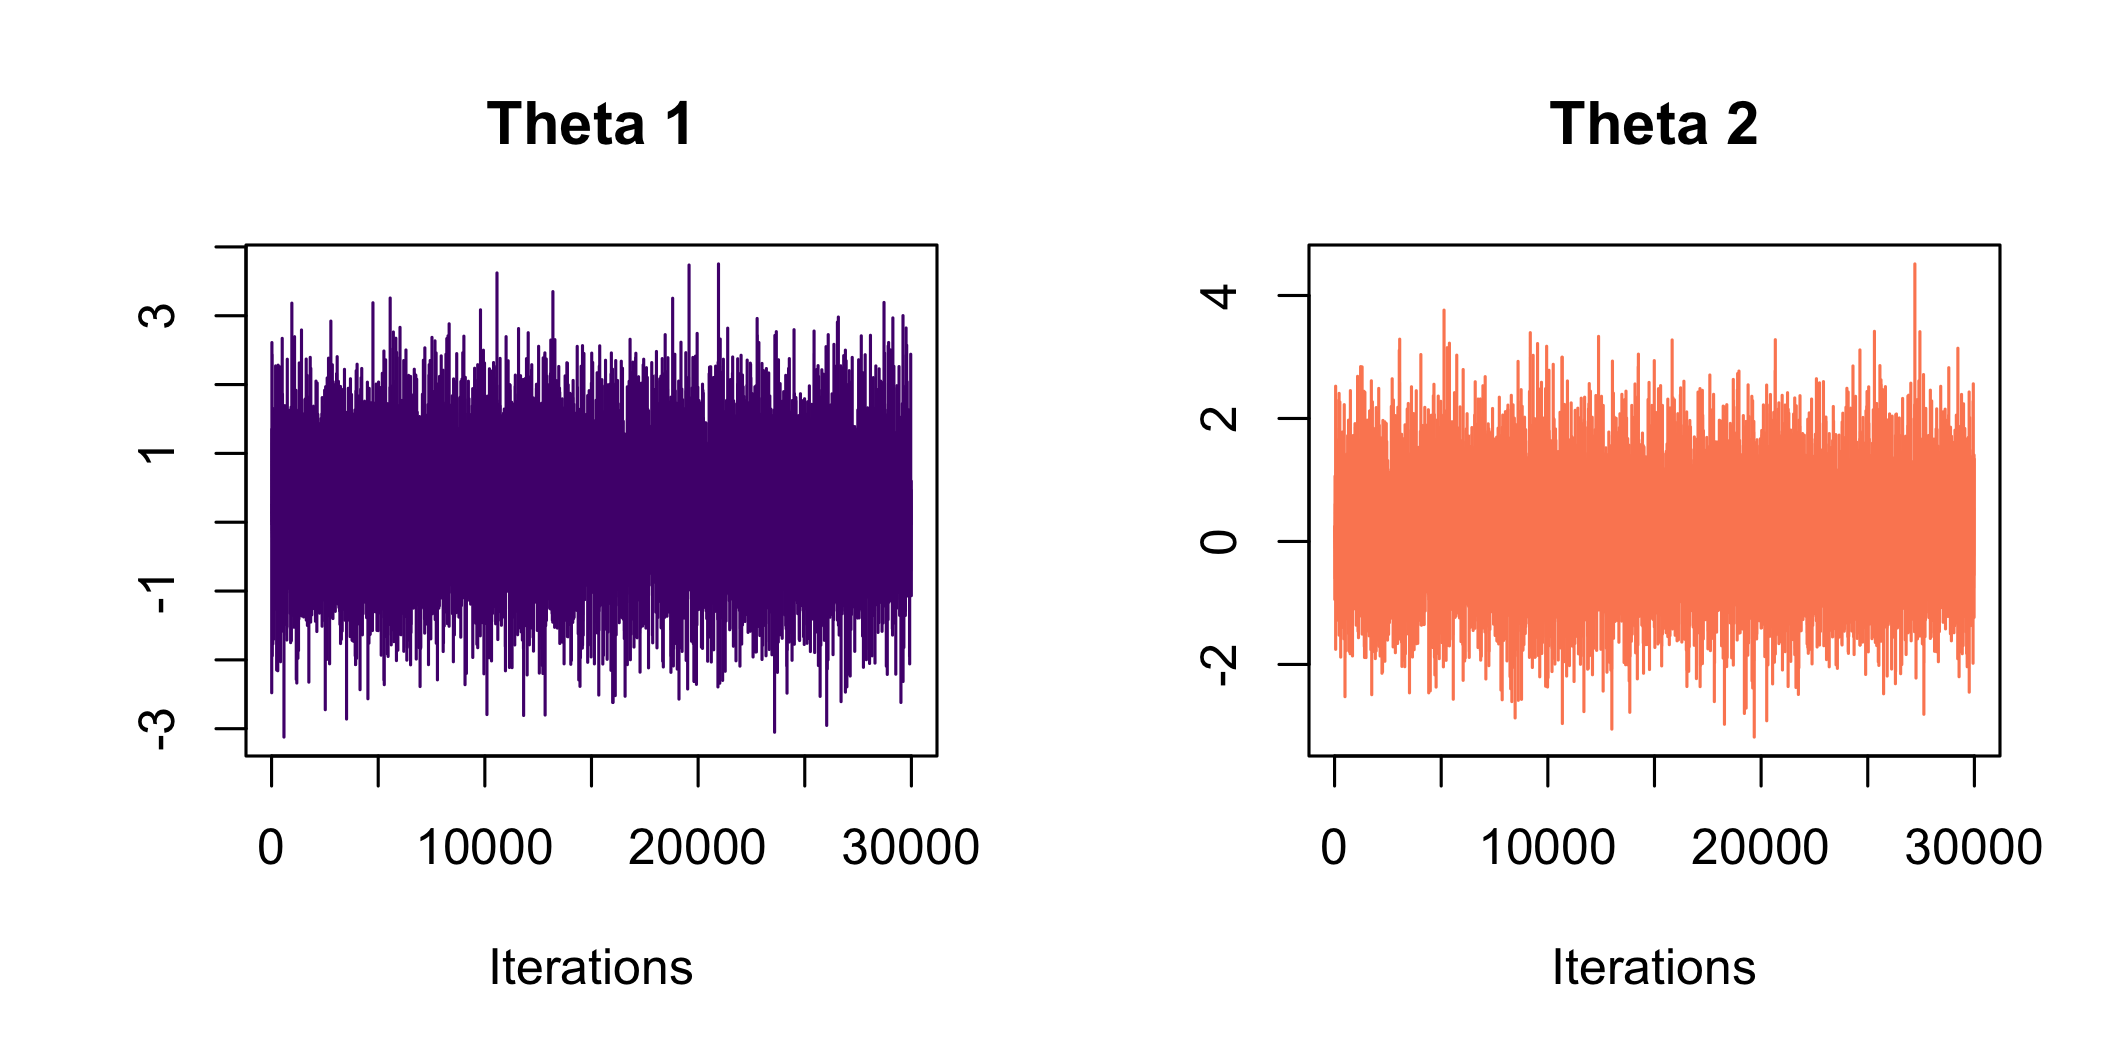
\includegraphics[width=0.6\linewidth]{pictures/fig01-gs-traceplot.png}
    \caption{Trace plots of $\theta_1$ and $\theta_2$ chains }
    \label{fig:gs-traceplot}
\end{figure}



\begin{table}[h!]
\centering
\caption{Summary statistics for Gibbs Sampler Chains.}
\begin{tabular}{lcccc}
\toprule
\textbf{} & \textbf{Mean} & \textbf{Median} & \textbf{95\% HPD Interval}  & \textbf{95\% Equal Tail} \\
\midrule
$\theta_1$ & 0.13877 & 0.09255 & [-1.192072, 1.657779] & [-1.208464, 1.643236] \\
$\theta_2$ & 0.10127 & 0.06755 & [-1.283651, 1.535148] & [-1.208464, 1.643236] \\
\bottomrule
\end{tabular}
\label{tab:summary_gs}
\end{table}

The acceptance rate of Gibbs sampling technique, based on full conditional distributions, is always 1(100\%). This is because every new value is sampled from the target distribution conditioned on valid values of all other variables $i.e$ the proposal distribution is the same as the full conditional distribution.
\subsection{Use the Geweke convergence diagnostic test on the generated chains and interpret your results.}
\subsubsection{Solution}
The Geweke test, is a formal convergence diagnostic test that assesses stationarity by comparing the means of the early (10\%) and late (50\%) portions of a Markov chain. From Table \ref{tab:geweke_gs} summaries, all $Z-score$ were within the acceptance region suggesting no evidence that the parameter mean of the late part is different from the early part. Figure \ref{fig:gs-geweke}   affirms the findings of the Geweke diagnostic test as the points fall within the acceptance window. We can there conclude that the chains likely achieved good convergence.
\begin{table}[h!]
\centering
\caption{Geweke convergence diagnostic test result}
\begin{tabular}{lcccc}
\toprule
\textbf{} & \textbf{1st window(\%)} & \textbf{2nd window(\%)} & \textbf{$Z-score$} & \textbf{Acceptance Interval($\alpha = 0.05$)}  \\
\midrule
$\theta_1$ & 0.1& 0.5 & -0.1207  & [-1.96, 1.96] \\
$\theta_2$ & 0.1& 0.5 & -0.8128 & [-1.96, 1.96] \\
\bottomrule
\end{tabular}
\label{tab:geweke_gs}
\end{table}

\begin{figure}[h!]
    \centering
    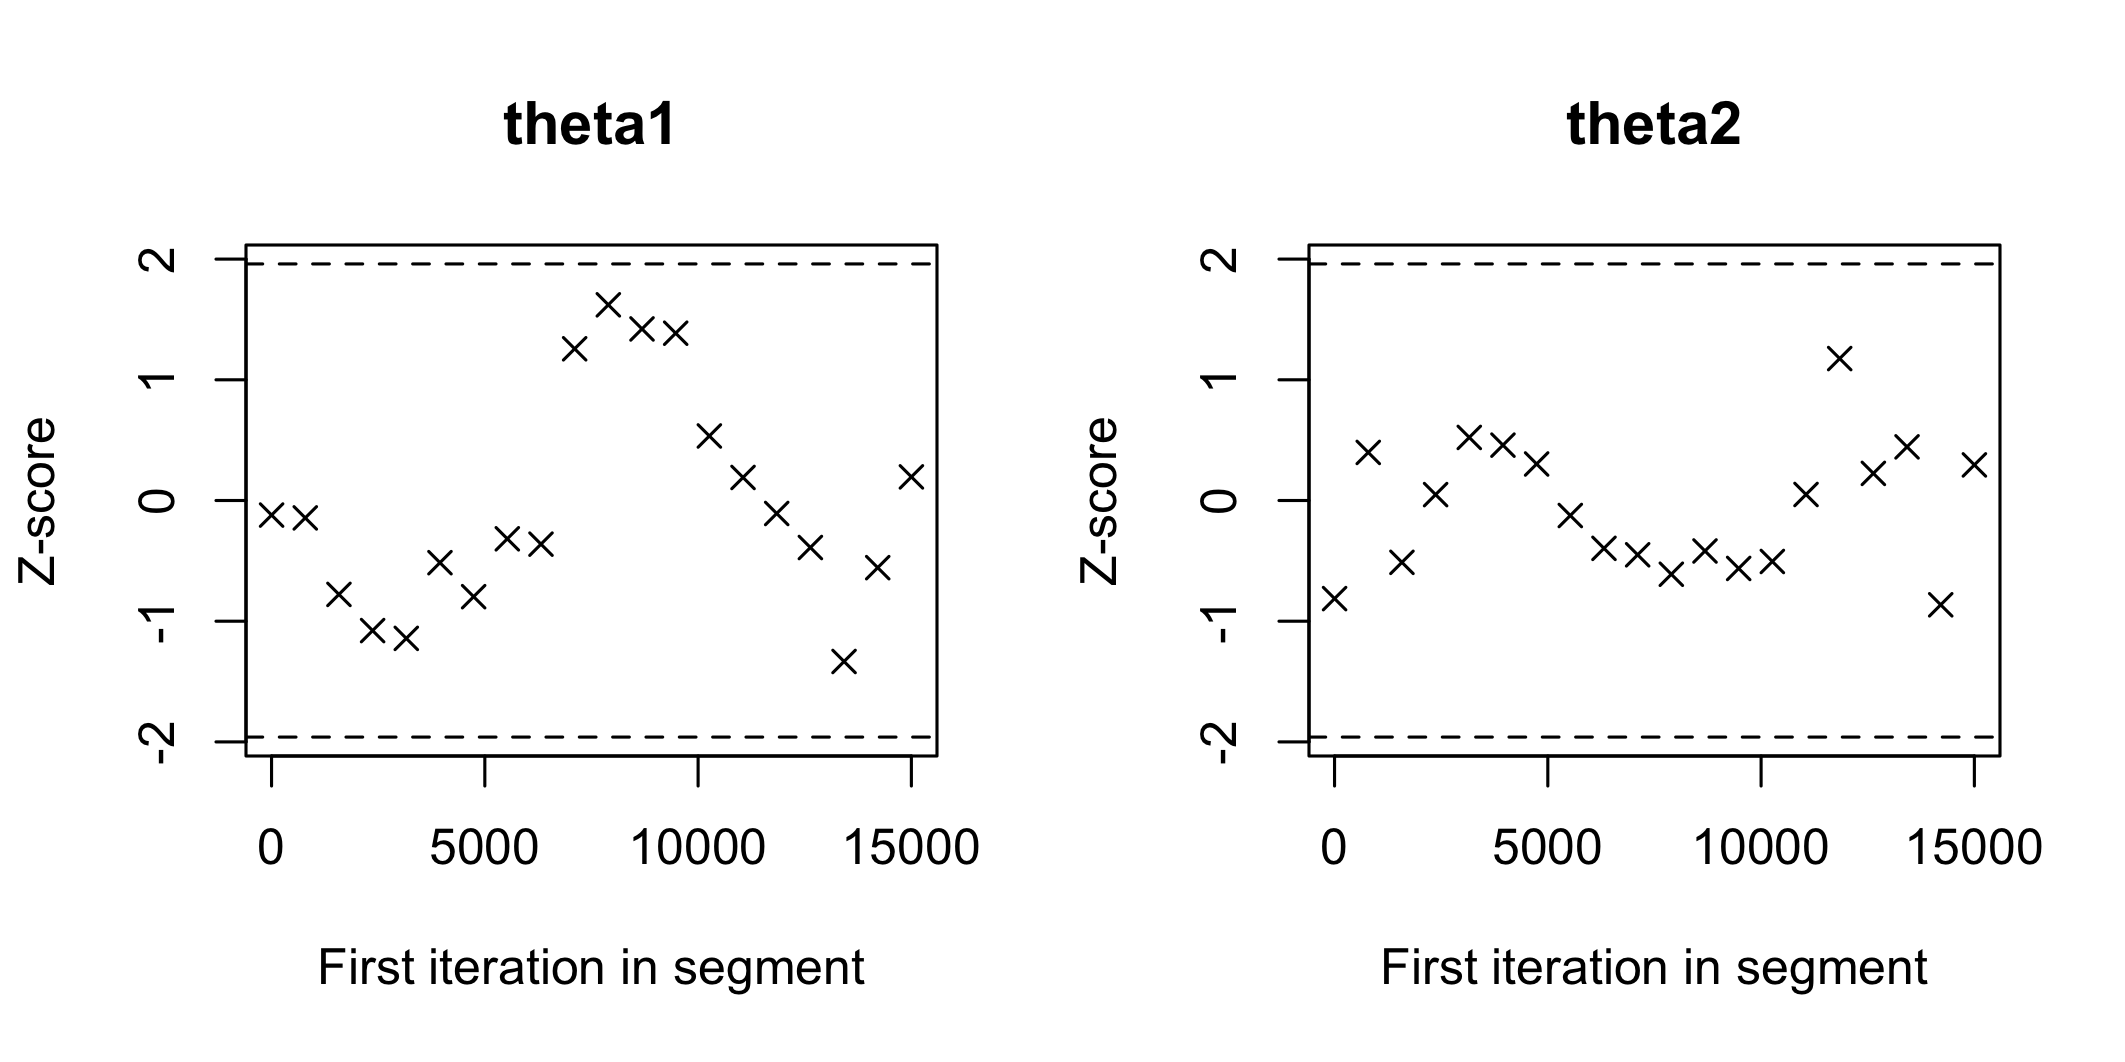
\includegraphics[width=0.6\linewidth]{pictures/fig05-gs-geweke.png}
    \caption{Geweke diagnostics plots for  $\theta_1$ and $\theta_2$ }
    \label{fig:gs-geweke}
\end{figure}


\subsection{Compute a point estimate for $\theta_1$ and a 95\% quantile-based credible interval}
\subsubsection{Solution}
Given the symmetric nature of $\theta_1$ values, either the mean and median could be sufficiently be used as a point estimate for $\theta_1$. As we can see from table \ref{tab:summary_gs}, the mean and the median of $\theta_1$ is 0.13877 and 0.09255 respectively. The 95\% equal tail is [-1.208464,1.643236].


\subsection{Using your generated chains, estimate the probability $P(\theta_1 > 0.5)$.}
\subsubsection{Solution}
The $p$ Monte Carlo value for which $p(\theta_1 > 0.5)$ was calculated as  $\frac{1 + \sum (\theta_1 > 0.5)}{30000 + 1}$ and found to be 0.2388587; $p(\theta_1 > 0.5)$ is thus 23.9 \%.


\section{Part 2 - The Metropolis algorithm}
\subsection{Write the log posterior distribution \( \log p(\theta|D) \) and obtain analytically the gradient
\[\nabla_\theta \log p(\theta|D) = \left( \frac{\partial \log p(\theta|D)}{\partial \theta_1}, \frac{\partial \log p(\theta|D)}{\partial \theta_2} \right)^\top \]
and Hessian matrix:
\[\nabla^2_\theta \log p(\theta|D) = 
\begin{pmatrix}
\frac{\partial^2 \log p(\theta|D)}{\partial \theta_1^2} & \frac{\partial^2 \log p(\theta|D)}{\partial \theta_1 \partial \theta_2} \\
\frac{\partial^2 \log p(\theta|D)}{\partial \theta_2 \partial \theta_1} & \frac{\partial^2 \log p(\theta|D)}{\partial \theta_2^2} 
\end{pmatrix}.\]}
\textbf{Solution}\\
The log posterior distribution could be written as:
\[
\log(p(\theta|D)) \propto -8\theta_1^2\theta_2^2 - 0.5\theta_1^2 - 0.5\theta_2^2 + \cos(2\pi + 0.3)\theta_1\theta_2 + 0.3\theta_1 + 0.2\theta_2
\]
By taking the first and second-order partial derivatives with regard to \(\theta_1\) and \(\theta_2\), of \(\log p(\theta|D)\),
we obtain the gradient as follows:
\[
\nabla_\theta \log p(\theta|D) = \left( -16\theta_1\theta_2^2 - \theta_1 + \cos(2\pi + 0.3)\theta_2 + 0.3, -16\theta_1^2\theta_2 - \theta_2 + \cos(2\pi + 0.3)\theta_1 + 0.2 \right)^\top
\]
And the Hessian matrix is as follows:
\[
\nabla^2_\theta \log p(\theta|D) = 
\begin{pmatrix}
-16\theta_2^2 - 1 & -32\theta_1\theta_2 + \cos(2\pi + 0.3) \\
-32\theta_1\theta_2 + \cos(2\pi + 0.3) & -16\theta_1^2 - 1
\end{pmatrix}
\]

\subsection{Using the gradient and Hessian matrix obtained in the previous step, implement a Newton-Raphson algorithm in R to find the posterior mode of \( p(\theta|D) \) and denote by
\[
\theta^*_{NR} = (\theta^*_1, \theta^*_2)^\top
\]
the mode after convergence of the algorithm. (Note: round \( \theta^*_{NR} \) to five digits after the decimal point).}
\textbf{Solution}\\
The Pseudo-code of Newton-Raphson algorithm to find the mode of \( p(\theta|D) \) is as follows:

\begin{algorithm}
\begin{algorithmic}[1]
\State Set tolerance \( \epsilon \), arbitrary initial distance \( d \), initialize \( \theta^{(0)} \) and set \( m = 0 \).
\While{$d > \epsilon$}
    \State \( \theta^{(m+1)} = \theta^{(m)} - \left( \nabla^2 \log p(\theta^{(m)}|D) \right)^{-1} \nabla \log p(\theta^{(m)}|D) \)
    \State Compute distance \( d = \|\theta^{(m+1)} - \theta^{(m)}\| \).
\EndWhile
\State At convergence, return \( \theta^M \).
\end{algorithmic}
\end{algorithm}

The following R code was implemented to obtain the posterior mode:

\lstset{
    language=R,
    basicstyle=\ttfamily\small,
    breaklines=true,
    breakatwhitespace=true,
    columns=fullflexible,
    backgroundcolor=\color{white},
    keywordstyle=\color{black},
    commentstyle=\color{black},
    stringstyle=\color{black},
    showstringspaces=false,
    numbers=left,
    numberstyle=\tiny\color{black}
}

\begin{lstlisting}
# define constants
A <- 16
B <- cos(2 * pi + 0.3)
C1 <- 0.3
C2 <- 0.2

# Define the gradient function in the global environment
gradient_theta <- function(theta = c(1, 2)) {
  t1 <- theta[1]
  t2 <- theta[2]
  grad1 <- -A * t1 * t2^2 - t1 + B * t2 + C1
  grad2 <- -A * t1^2 * t2 - t2 + B * t1 + C2
  return(c(grad1, grad2))
}

# Define the Hessian function in the global environment
hessian_theta <- function(theta = c(1, 2)) {
  t1 <- theta[1]
  t2 <- theta[2]
  h11 <- -A * t2^2 - 1
  h12 <- h21 <- -2 * A * t1 * t2 + B
  h22 <- -A * t1^2 - 1
  return(matrix(c(h11, h12, h21, h22), nrow = 2))
}

NewtonRaphson <- function(theta0 = c(1, 2), tolerance = 1e-10, iteration = 1000) {
  for (i in 1:iteration) {
    grad_theta0 <- gradient_theta(theta0)
    hes_theta0 <- hessian_theta(theta0)
    theta1 <- theta0 - solve(hes_theta0, grad_theta0) # Calculate next value of theta
    distance <- sum(abs(theta1 - theta0))
    if (distance < tolerance) { # Once distance between theta1 and theta0 gets sufficiently small, output result
      result <- round(theta1, 5)
      return(list("mode theta" = result, paste("Converged at iteration", i)))
    }
    # If convergence not reached, set theta1 as theta0 and continue
    theta0 <- theta1
  }
  print('Newton-Raphson algorithm did not converge. Choose a larger number of iterations.')
}

theta_NR_star <- NewtonRaphson()$'mode theta'
theta_NR_star

\end{lstlisting}
Using the above algorithm, the posterior mode of \( p(\theta|D) \) was found to locate at
\[ \theta^*_{NR} = (0.2997; 0.1996)^\top \]

\subsection{Compute a Laplace approximation to \( p(\theta|D) \) around \( \theta^*_{NR} \). Report the covariance matrix \( \Sigma^* \) of the Laplace approximation. (Note: round your results to five digits after the decimal point).}
\textbf{Solution}\\
Using Laplace approximation around \( \theta^*_{NR} \), the posterior distribution \( p(\theta|D) \) is approximated
by a Gaussian distribution with
\begin{itemize}
    \item Mean \( \mu^{0} = \theta^*_{NR} - (\nabla^2 \log p(\theta^*_{NR}|D))^{-1} \nabla \log p(\theta^*_{NR}|D) \)
    \item Covariance matrix \( \Sigma^* = (\nabla^2 \log p(\theta^*_{NR}|D))^{-1} \)
\end{itemize}
With \( \nabla \log p(\theta^*_{NR}|D) \) and \( \nabla^2 \log p(\theta^*_{NR}|D))^{-1} \) the gradient and Hessian, respectively, of the
log target posterior distribution, evaluated at \( \theta^*_{NR} \).

Using the calculation from Question 1, the covariance matrix \( \Sigma^* \) is:
\[ \Sigma^* =
\begin{pmatrix}
0.7935 & -0.3121 \\
-0.3121 & 0.5330
\end{pmatrix}
\]

And the mean \( \mu^{0} \):
\[ \mu^{0} =
\begin{pmatrix}
0.2997 \\
0.1996
\end{pmatrix}
\]

Thus the distribution of the approximated posterior distribution is:
\[ \tilde{p}_G(\theta|D) \sim N\left(
\begin{pmatrix}
0.2997 \\
0.1996
\end{pmatrix}
,
\begin{pmatrix}
0.7935 & -0.3121 \\
-0.3121 & 0.5330
\end{pmatrix}
\right) \]

\subsection{In R, write a random-walk Metropolis algorithm to explore the joint posterior \( p(\theta|D) \) using a Gaussian proposal with covariance matrix \( \tilde{\Sigma} = c\Sigma^* \). Use a chain of length \( M = 50,000 \) and tune \( c \) to (approximately) reach the optimal acceptance rate of 23\%. Please specify \textit{set.seed(1993)} for the sake of reproducibility of your results.}
\textbf{Solution}\\
The pseudo-code of the random-walk Metropolis algorithm is as follows:
\begin{enumerate}
    \item Choose initial value \( \theta^{0} \) satisfying \( p(\theta^{0}|D) > 0 \)
    \item For \( m \) in 1 to \( M \) do:
    \begin{enumerate}
        \item Sample \( \tilde{\theta}^{(m)} \sim q(\cdot|\theta^{(m-1)}) \)
        \item Compute the log ratio \( \log \varrho(\theta^{(m-1)}, \tilde{\theta}^{(m)}) = \log \frac{p(\tilde{\theta}^{(m)}|D)}{p(\theta^{(m-1)}|D)} \)
        \item Sample \( u \sim U(0, 1) \)
        \item If $\log(\varrho) \geq 0 \; \| \; u \leq \exp(\log(\varrho))$, set $\theta^{(m)} \gets \tilde{\theta}^{(m)}$ (accept candidate)
        \item Else \( \theta^{(m)} \leftarrow \theta^{(m-1)} \) (reject candidate)
    \end{enumerate}
    \item End for.
\end{enumerate}

The following Metropolis algorithm was implemented in R to explore \( p(\theta|D) \):

\begin{lstlisting}
Metropolis <- function(M = 51000, burn_in = 1000, seed = 1993, 
                       theta_start = c(0.29970, 0.19955), c_tune = 2 )
{
  set.seed(seed)
  
  # Joint log posterior distribution
  log_posterior <- function(theta)
  {
    t1 <- theta[1]
    t2 <- theta[2]
    return(-1/2*(A*t1^2*t2^2 + t1^2 + t2^2 - 2*B*t1*t2 - 2*C1*t1 - 2*C2*t2))
  }
  
  # Starting value for theta 1 and theta 2
  theta <- array(dim = c(2, M))
  theta[, 1] <- theta_start
  n_accept <- 0
  
  # Gaussian proposal
  # Covariance matrix
  theta_NR_star <- NewtonRaphson()$'mode theta' #The NewtonRaphson function built in Q2
  sigma_star <- round(solve(-hessian_theta(theta = theta_NR_star)),5)
  sigma_tilde <- c_tune*sigma_star
  
  # Metropolis loop
  for (i in 2:M)
  {
    # New proposed theta
    theta_prop <- theta[,i - 1] + rmvnorm(n = 1, 
                                        mean = c(0,0), sigma = sigma_tilde)
    # Log ratio for accept-reject decision
    logr <- log_posterior(theta_prop) - log_posterior(theta[,i - 1])
    
    # Accept or reject
    u <- runif(1)
    if (logr >= 0 || u <= exp(logr))
    { #Accept
      theta[,i] <- theta_prop
      n_accept <- n_accept + 1
    } 
    else 
    { #Reject, stay where theta is
      theta[,i] <- theta[, i - 1]
    }
  }
  # Exclude burn-in
  theta <- theta[,-c(1:burn_in)]
  # Output
  accept_rate <- round(n_accept/(M - 1), digits = 3) * 100
  rownames(theta) <- c("Theta1","Theta2")
  output <- list(theta = theta,
                 M = M, 
                 burn_in = burn_in,
                 log_posterior = log_posterior)
  print(paste("Acceptance rate:", accept_rate,"%"))
  return(invisible(output))
}

MCMC_run <- Metropolis(c_tune = 2.8)

\end{lstlisting}

Our MCMC chain had 51000 iterations; the first 10000 were burn-in period. The
starting point of \( \theta \) was set at \( \theta^*_{NR} \). The tuning factor \( c \) was set at 2.8 to give the acceptance
rate of 23.3\%. The trace plots, Q-Q plots, running mean plots, and Geweke diagnostic (Figure
\ref{fig:mh-traceplot}, \ref{fig:mh-qqplot}, \ref{fig:mh-runmean}, and \ref{fig:mh-geweke}) showed good signs of convergence.

\begin{figure}[H]
    \centering    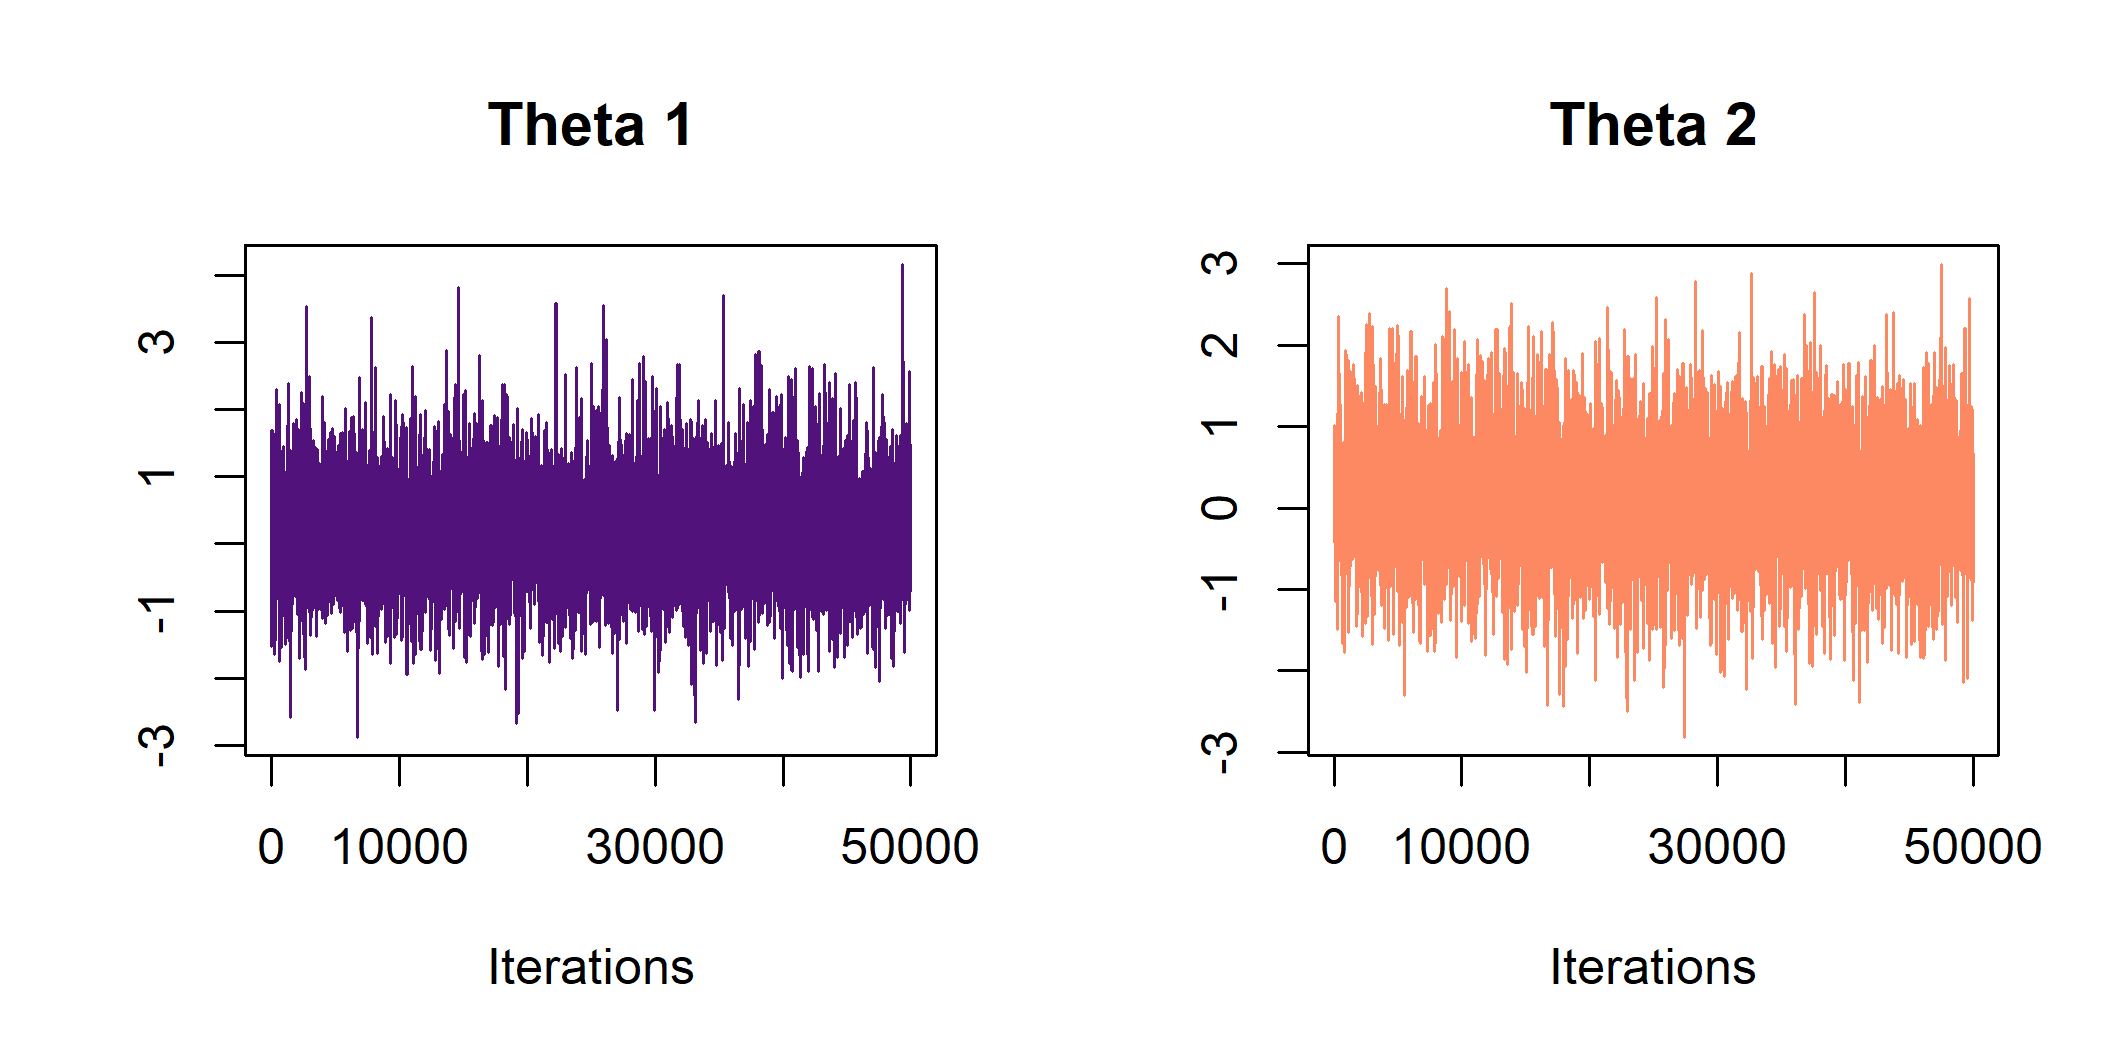
\includegraphics[width=0.8\textwidth]{pictures/fig01-mh-traceplot.png}
    \caption{Trace plots of \( \theta_1 \) and \( \theta_2 \)}
    \label{fig:mh-traceplot}
\end{figure}

\begin{figure}[H]
    \centering    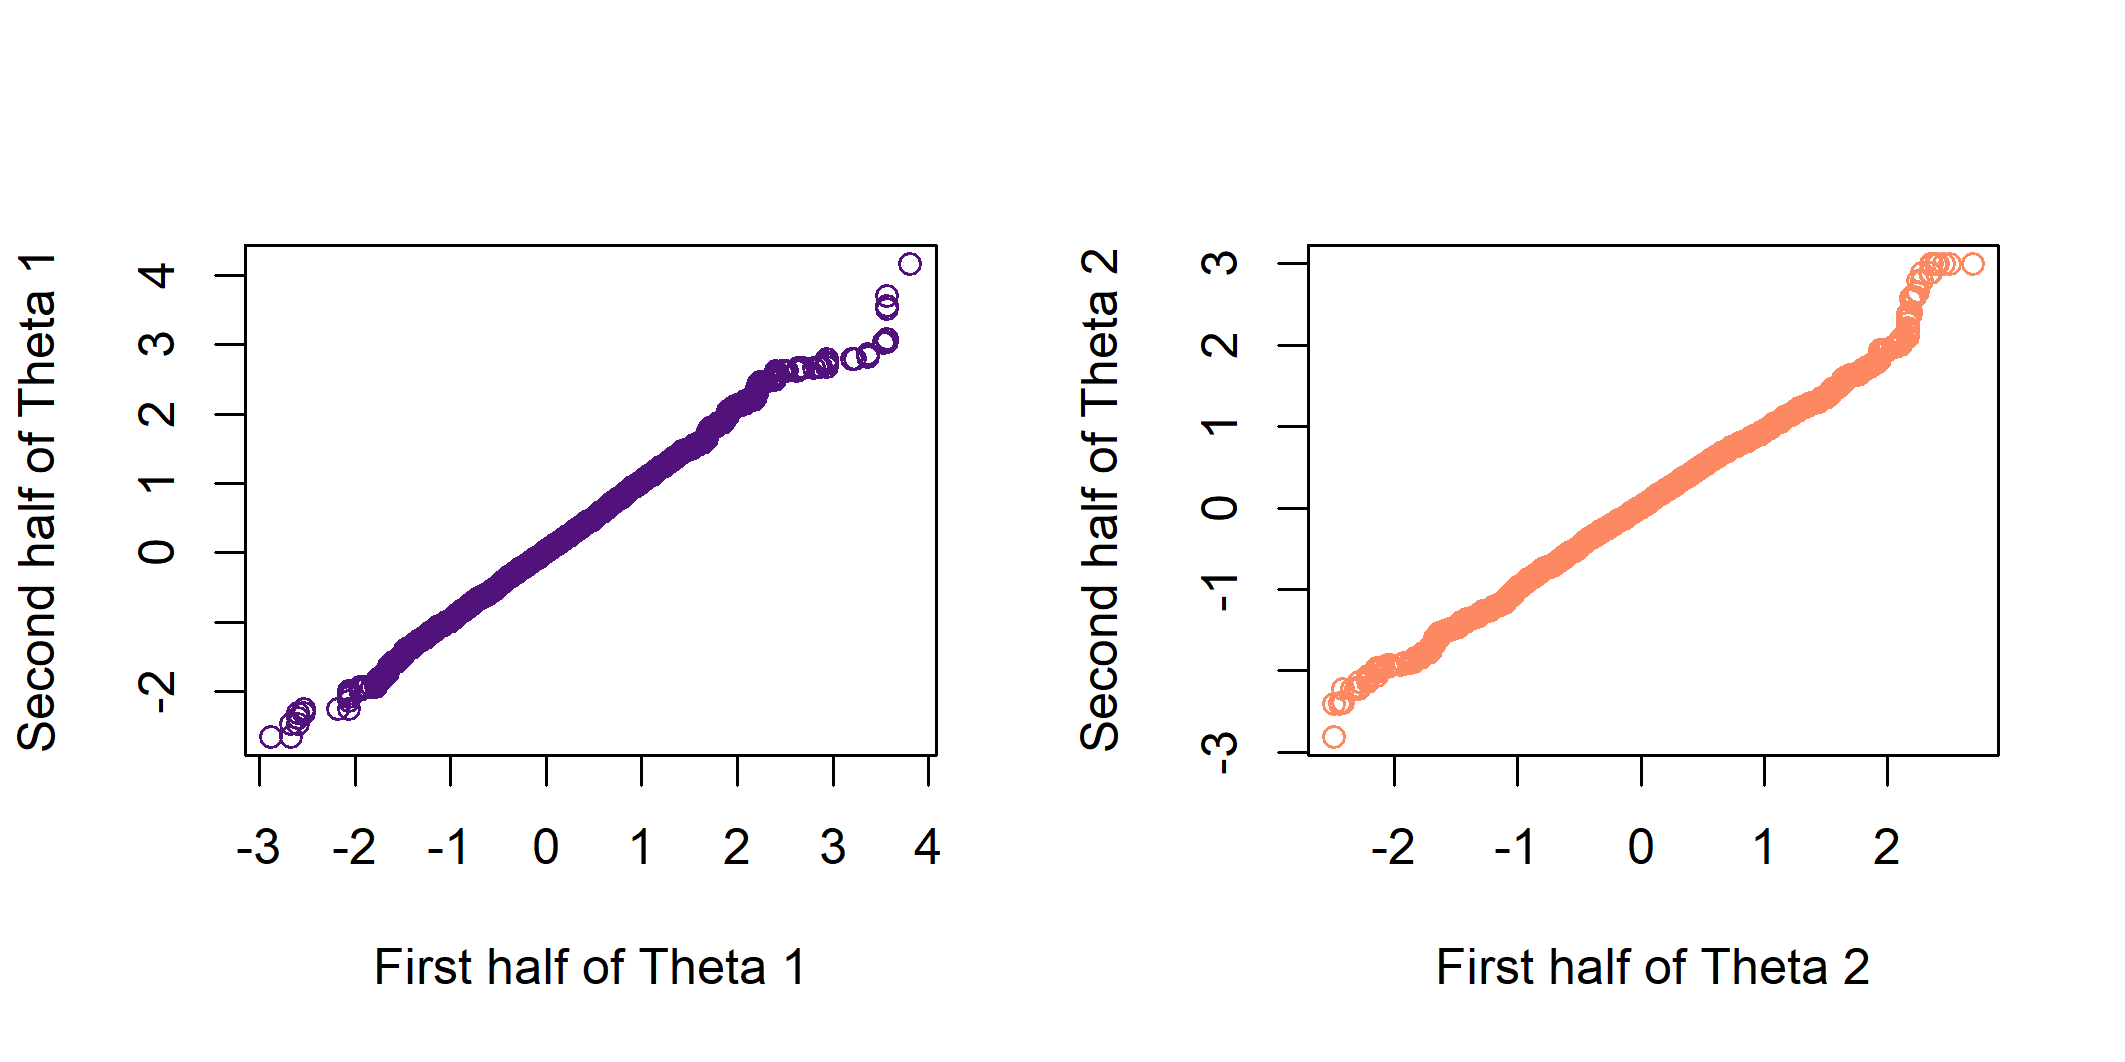
\includegraphics[width=0.8\textwidth]{pictures/fig03-mh-qqplots.png}
    \caption{Q-Q plots of \( \theta_1 \) and \( \theta_2 \)}
    \label{fig:mh-qqplot}
\end{figure}

\begin{figure}[H]
    \centering    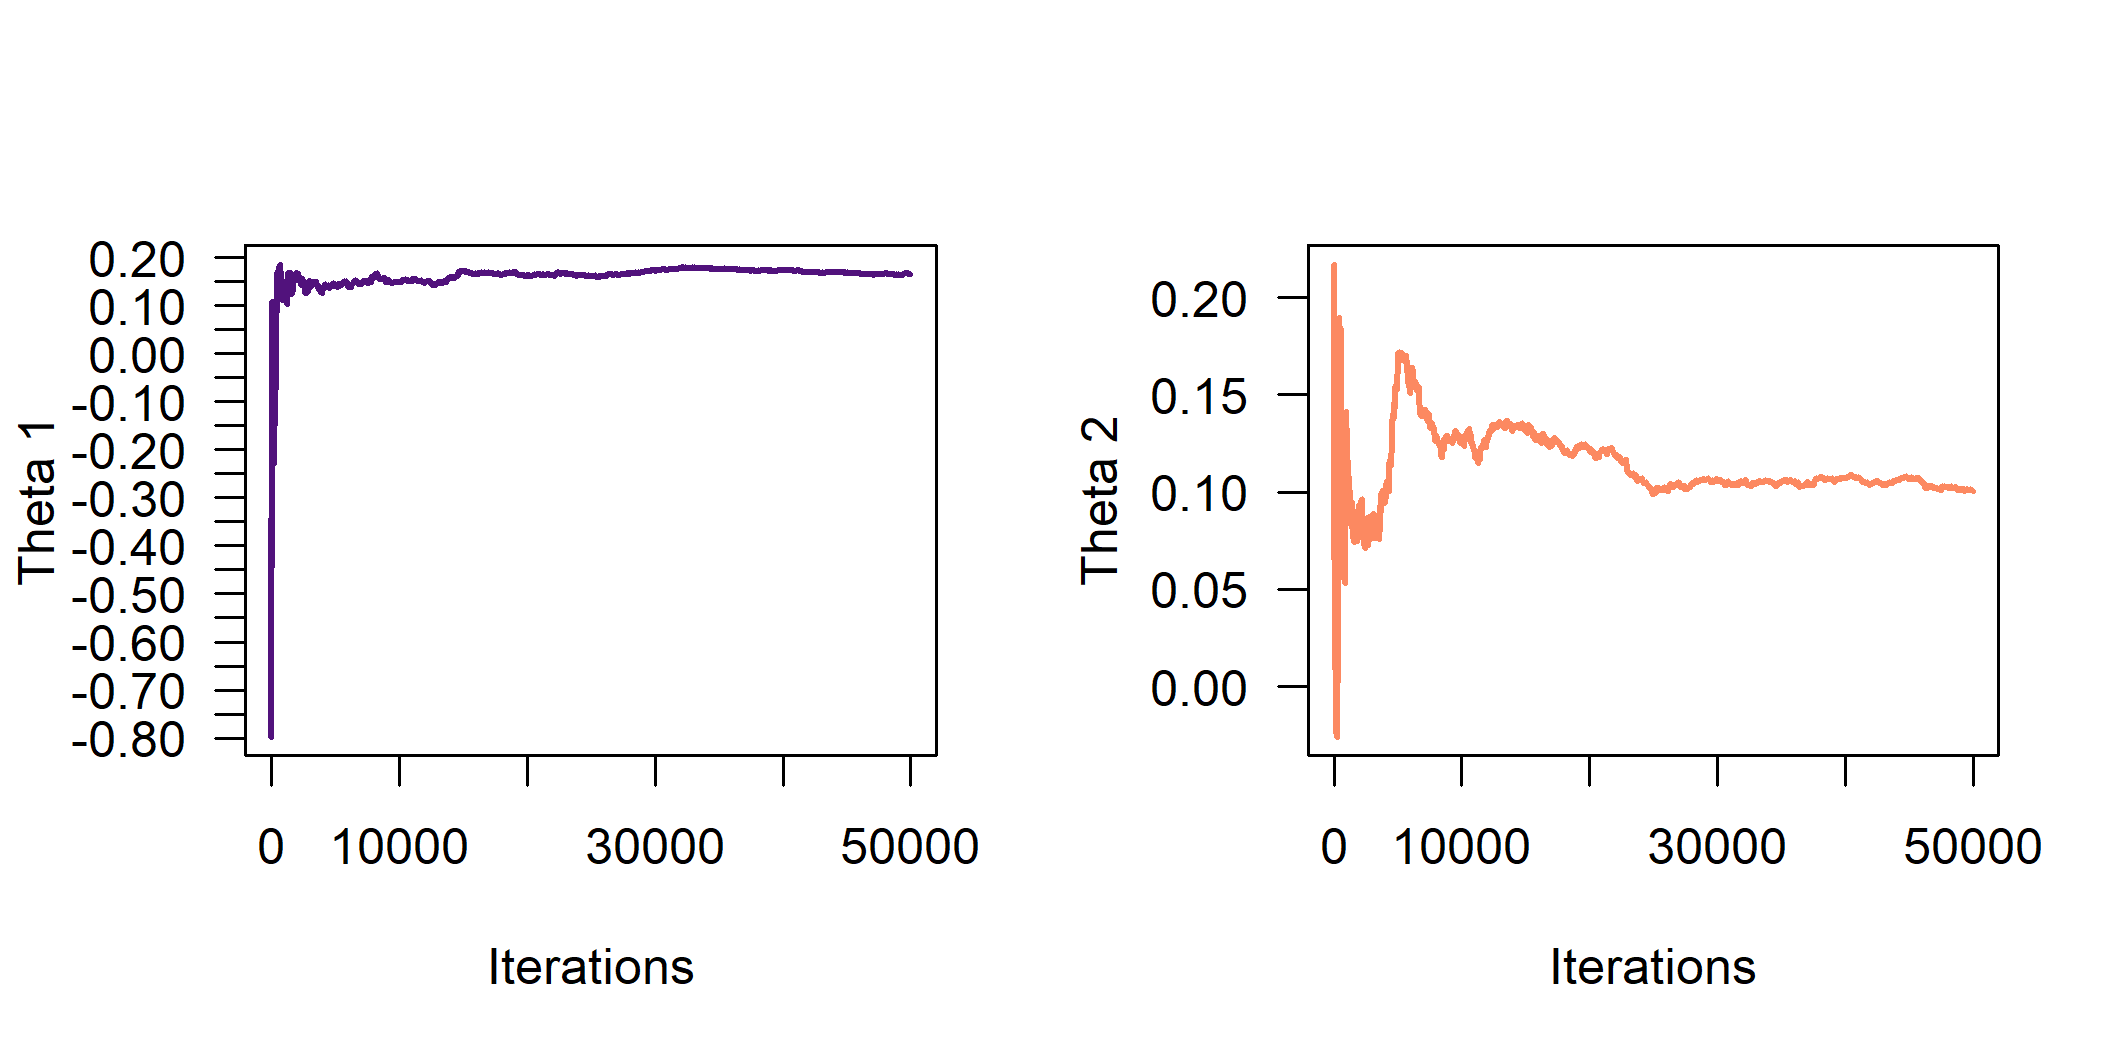
\includegraphics[width=0.8\textwidth]{pictures/fig04-mh-runmean.png}
    \caption{Running mean plots of \( \theta_1 \) and \( \theta_2 \)}
    \label{fig:mh-runmean}
\end{figure}

\begin{figure}[H]
    \centering    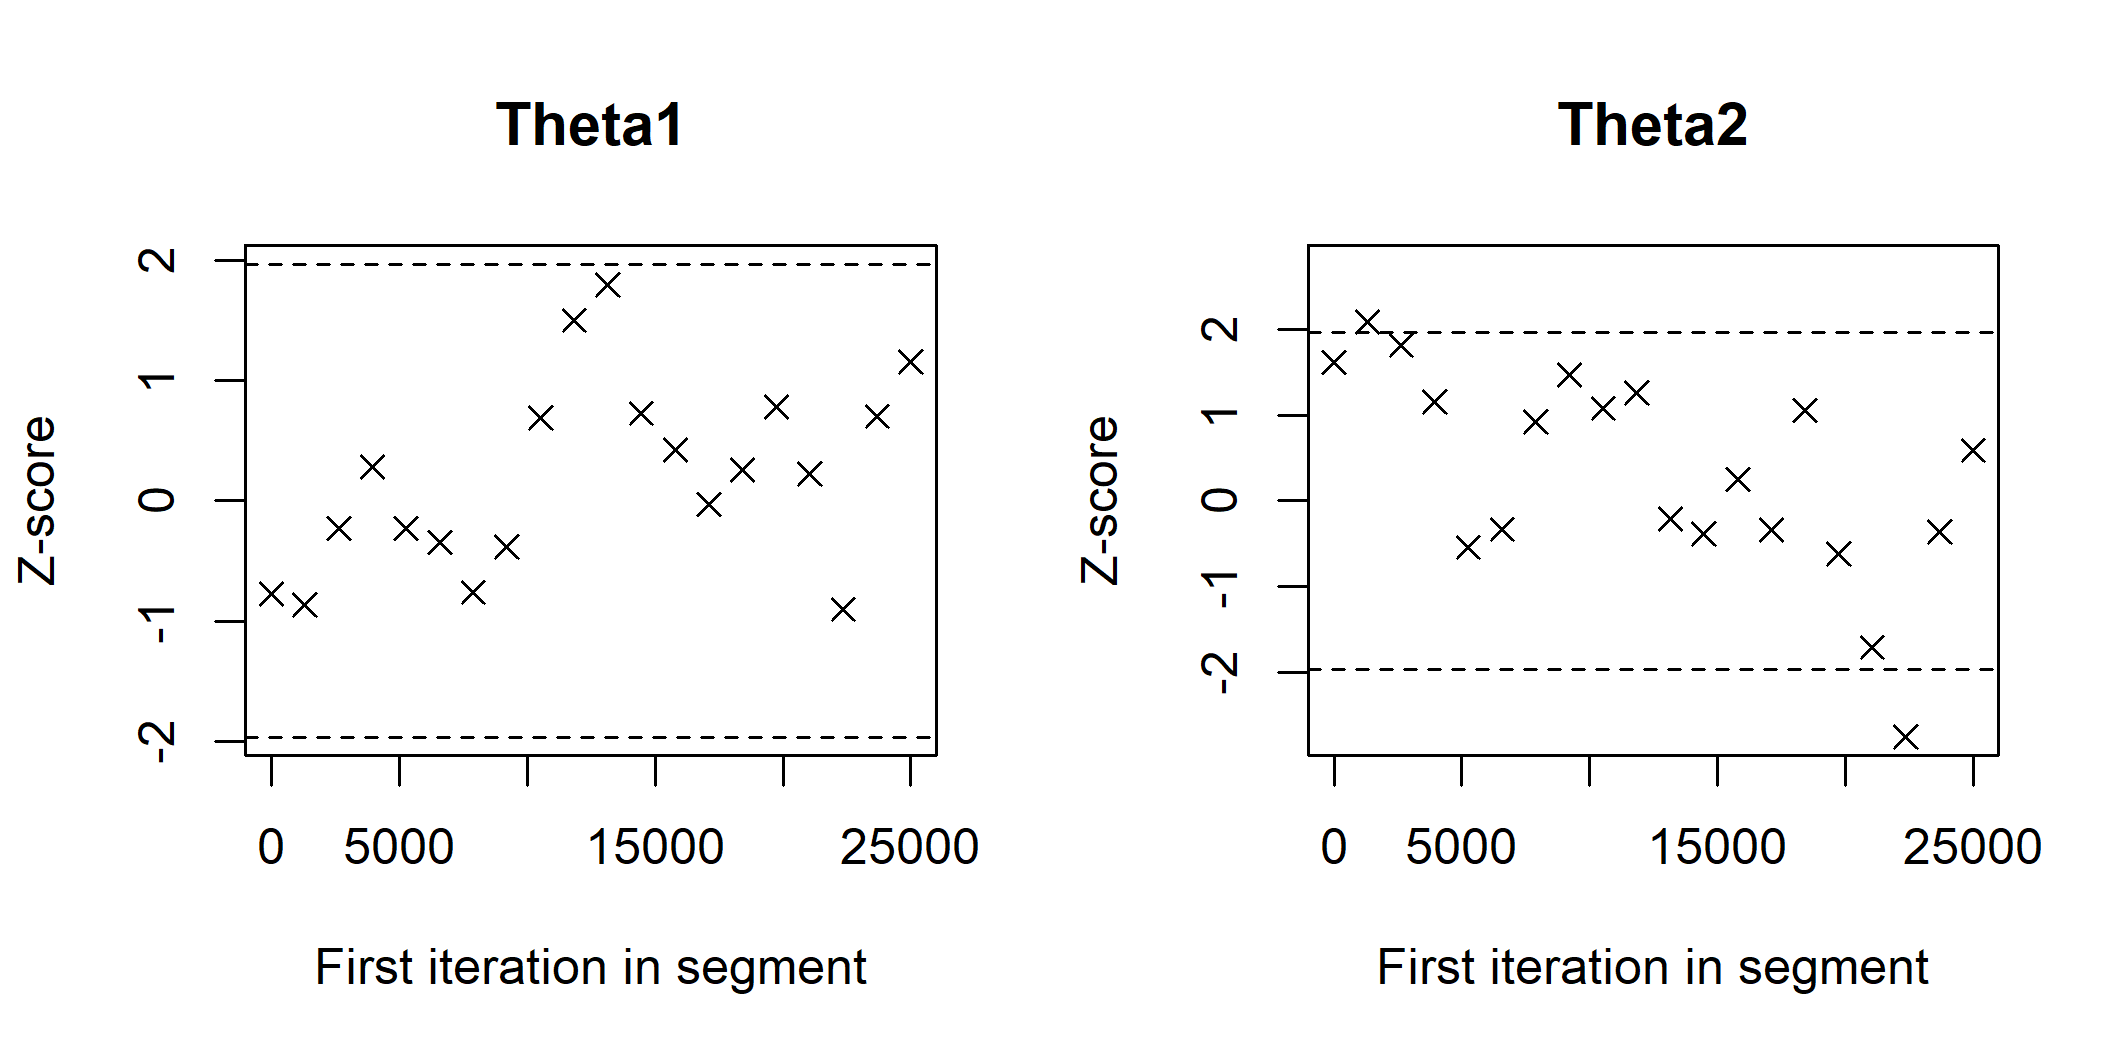
\includegraphics[width=0.8\textwidth]{pictures/fig05-mh-geweke.png}
    \caption{Time series plots of Geweke test statistic for \( \theta_1 \) and \( \theta_2 \)}
    \label{fig:mh-geweke}
\end{figure}

The summary statistics of posterior $\theta_1$ and $\theta_2$ is given in Table \ref{tbl:mh-summary}.

\begin{table}[H]
\centering
\begin{tabular}{lcccccc}
\hline
Parameter & Posterior mean & Posterior median & Posterior SD & 95\% equal tail CI & 95\% HPD interval \\
\hline
$\theta_1$ & 0.165 & 0.084 & 0.686 & -1.101 ; 1.726 & -1.101 ; 1.723 \\
$\theta_2$ & 0.101 & 0.066 & 0.648 & -1.210 ; 1.579 & -1.231 ; 1.548 \\
\hline
\end{tabular}
\caption{Summary measures of the posterior distribution of $\theta_1$ and $\theta_2$}
\label{tbl:mh-summary}
\end{table}

\subsection{Using your generated chains, estimate the probability \( P\left(\frac{\theta_1}{\theta_2} > 0.45\right) \).}
\textbf{Solution}\\
The probability \( P\left(\frac{\theta_1}{\theta_2} > 0.45\right) \) was calculated as the proportion of the MCMC chain that produced the ratio \( \frac{\theta_1}{\theta_2} > 0.45 \). It was estimated to be 0.374.

\printbibliography

\end{document}
